\documentclass[12px]{article}

\title{Lezione 2 Metodi Numerici}
\date{2026-03-03}
\author{Federico De Sisti}

\input{../../setup.tex}

\begin{document}
	\maketitle
	\newpage
	\subsection{boh}
	\[
	\begin{cases}
		\dot y(t) = y(t)\ \ \ \ t > 0 \\
		y(0) = y_0
	\end{cases}
	.\] 
	$y:[0,+\infty) \Rightarrow \R$ \\
	$y(t) = y_0e^t$ è soluzione del sistema\\
	$y(t_{n+1}) - y(t_n) = y_0e^{t_{n+1}} - y_0e^{t_n} = y_0e^{t_n}(e^{\Delta t} - 1)> 0$ se $y_0 > 0$, quindi due elementi successivi si allontanano sempre di più.\\
	Bisogna ora trovare gli equilibri, ovvero i punti in cui la dinamica si annulla.\\
	Come campo abbiamo $P(Y) = Y = \dot Y$\\
	Vogliamo quindi  $P(Y) = 0 \Rightarrow \begin{cases}
		\dot Y = 0\\
		Y_0 \ \ t.c.\ \  P(Y_0) = 0
	\end{cases}$ 
	Questo si annulla solamente nell'origine.\\
	Guardando lo spazio degli stati, se sono a destra dell'origine ho velocità positiva, se sono a sinistra ho velocità negativa, questo equilibrio è quindi instabile.\\
\begin{figure}[h]
    \centering
    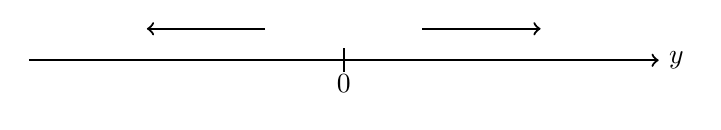
\begin{tikzpicture}

        % 1. Disegna la retta orizzontale orientata (asse principale)
        \draw[->, thick] (-4,0) -- (4,0) node[right] {$y$};

        % 2. Segna lo zero con una piccola tacca verticale
        \draw[thick] (0,-0.15) -- (0,0.15) node[below=0.2cm] {$0$};

        % 3. Freccia a destra che punta verso lo zero (es. limite da destra)
        \draw[->, thick]  (1, 0.4) -- (2.5, 0.4);

        % 4. Freccia a sinistra che punta verso lo zero (es. limite da sinistra)
        \draw[->, thick]  (-1, 0.4)--(-2.5, 0.4);

    \end{tikzpicture}
    \caption{Equilibrio Instabile}
\end{figure}

	Prendiamo ora in considerazione $ \begin{cases}
		\dot Y = -Y\\
		Y(0) = Y_0
	\end{cases}$ che ha soluzione \\
	$Y(t) = y_0e^{-t}$ \\
	\documentclass{article}
\usepackage{tikz}

\begin{document}

\begin{figure}[h]
    \centering
    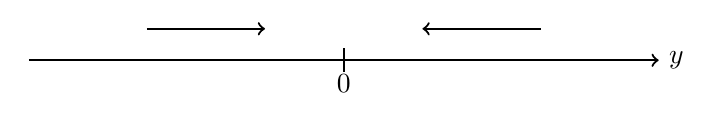
\begin{tikzpicture}

        % 1. Disegna la retta orizzontale orientata (asse principale)
        \draw[->, thick] (-4,0) -- (4,0) node[right] {$y$};

        % 2. Segna lo zero con una piccola tacca verticale
        \draw[thick] (0,-0.15) -- (0,0.15) node[below=0.2cm] {$0$};

        % 3. Freccia a destra che punta verso lo zero (es. limite da destra)
        \draw[->, thick] (2.5, 0.4) -- (1, 0.4);

        % 4. Freccia a sinistra che punta verso lo zero (es. limite da sinistra)
        \draw[->, thick] (-2.5, 0.4) -- (-1, 0.4);

    \end{tikzpicture}
    \caption{Equilibrio Stabile}
\end{figure}
Prendiamo ora in considerazione il sistema della mappa logistica
\[
\begin{cases}
	\dot y = y(1-y) = f(y)\\
	y(0) = 0
\end{cases}
.\] 
Questo ha due punti di equilibrio, $y_0 = 0$ e $y_0 = 1$ tali che $f(y) = 0$\\
Proviamo ora a sviluppare con Taylor attorno ai punti di equilibrio, al primo ordine, avendo così un approssimazione lineare.
\[
	f(y) = y(1-y) = y - y^2 \ \ \substack{\text{vicino a 0}\\\sim} \ \ y
.\] 
Ma questo è un caso che sappiamo trattare\\
    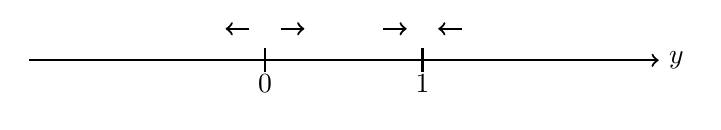
\begin{tikzpicture}

        % 1. Disegna la retta orizzontale orientata (asse principale)
        \draw[->, thick] (-4,0) -- (4,0) node[right] {$y$};

        % 2. Segna lo zero con una piccola tacca verticale
        \draw[thick] (-1,-0.15) -- (-1,0.15) node[below=0.2cm] {$0$};
        \draw[thick] (1,-0.15) -- (1,0.15) node[below=0.2cm] {$1$};

        % 3. Freccia a destra che punta verso lo zero (es. limite da destra)
        \draw[->, thick]  (-0.8, 0.4) -- (-0.5, 0.4);

        % 4. Freccia a sinistra che punta verso lo zero (es. limite da sinistra)
        \draw[->, thick]  (-1.2, 0.4)--(-1.5, 0.4);

        \draw[->, thick]  (0.5, 0.4) -- (0.8, 0.4);

        % 4. Freccia a sinistra che punta verso lo zero (es. limite da sinistra)
        \draw[->, thick]  (1.5, 0.4)--(1.2, 0.4);
    \end{tikzpicture}
    \[
    f(y) \sim f(y_1) + f'(y_1)(y-y_1) + O(|y-y_1|)
    .\] 
    \[
     = 0 + (1 - 2y_1)(y-y_1) + O(|y-y_1|) = -(y-1) = 1-y
    .\] 
    INSERISCI Foto della soluzionea 3 marzo 1:57
    \subsection{Stabilità alla variabile}
    Prendo il solito sistema
    \[
	    \begin{cases}
	    \dot y(t) = f(t,y(t)) \ \ t\in [0,T]\\
	    y(0) = y_0
    \end{cases}
    .\] 
    Chiamo ODE$\delta$ il seguente sistema perturbato
    \[
    \begin{cases}
	    \dot z(t) = f(t,z(t) + \delta(t)) \ \ t\in [0,T]\\
	    z(0) = y_0 + \delta_0
    \end{cases}
    .\] 
    Trovato poiché abbiamo perturbato gli unici due dati del problema, questo può capitare, possiamo vederlo come l'errore causato da uno strumento.\\
    \begin{defi}[Stabilità di Lyapunov]
    ODE è stabile in senso Lyapunov su $(0,T)$ se  $\forall \delta_0$ e $\forall \delta(t)$ tali che  $|\delta_0|< \varepsilon \ \ \ |\delta(t)| < \varepsilon$ per $t\in(0,T)$ con  $\varepsilon > 0$ tale ODE$\delta$ ha  soluzione
    \[
    \exists C > 0 \ \ t.c. |y(t)-z(t)|<C\varepsilon \ \ \forall t\in (0,T)
    .\] 
    \end{defi}
MI RACCOMANDO NON LA SBAGLIARE, ATTENTO AI QUANTIFICATORI \\
Ciò sta a significare che se perturbo poco, le soluzioni sono abbastanza vicine.\\
\begin{defi}
Se $T \rightarrow +\infty$ diciamo che ODE è asintoticamente stabile se:
\begin{enumerate}
	\item è stabile in senso Lyapunov $\forall T> 0$
	\item $|y(t) - z(t)| \xrightarrow{ t \rightarrow +\infty}0$ se $|\delta(t)| \xrightarrow{t \rightarrow+\infty}0$
\end{enumerate}
\end{defi}
\textbf{Esempio:}\\
\[
\begin{cases}
	\dot y = y\\
	y(0) = y_0
\end{cases} \rightarrow \ y(t) = y_0e^t
.\] 
Perturbiamo il sistema nel modo più semplice, perturbiamo il dato iniziale
\[
	\begin{cases}
\dot z = z\\
z(0) = y_0 + \delta_0
	\end{cases}
.\] 
Che ha soluzione $z(t) = (y_0 + \delta_0)e^t$\\
\[
|z(t) - y(t)| = |(y_0 + \delta_0)e^t - y_0e^t| = |\delta_0 e^t| = |\delta_0|e^t\leq |\delta_0|e^T
.\] 
Chiamo $C = e^T$ e ottengo
 \[
|z(t) -y(t)| \leq |\delta_0|C\leq C \varepsilon
.\] 
Ma $e^T$ è enorme, ciò vuol dire che regolare l'errore devo prendere un  $\varepsilon$ minuscolo.\\
La distanza tuttavia non tende a $0$ se $t \rightarrow +\infty$, quindi non abbiamo stabilità asintotica.\\
Quindi questo è stabile in senso di Lyapunov ma non asintoticamente stabile.\\
\textbf{Esempio:}
\[
\begin{cases}
	\dot y = -y\\
	y(t) = y_0
\end{cases} \rightarrow y(t) = y_0e^{-t}
.\] 
\[
\begin{cases}
	\dot z = -z\\
	z(t) = y_0 + \delta_0
\end{cases}
.\]
E otteniamo così
\[
	|z(t) - y(t)| = |\delta_0e^{-t}| = |\delta_0|e^{-t}\leq |\delta_0|= C\varepsilon
.\] 
con $C = 1$
\begin{lemm}[di Gronwall]
	Sia $p$ una funzione integrabile e non negativa su $(0,T)$  e siano  $g, \varphi$ funzioni continue su $[0,T]$ con  $g$ non decrescente.\\
	Se $ \varphi$ soddisfa $ \varphi(t) \leq g(t) + \int_0^Tp(s) \varphi(s)ds \ \ \forall t\in [0,T]$\\
	allora
	\[
		\varphi(t)\leq g(t)e^{\int_0^t \varphi(s) ds} 
	.\] 
\end{lemm}
La dimostrazione è noiosa e la puoi cercare su wikipedia.\\
Considero
\[
\begin{cases}
	\dot y = f(y(t))\\
	y(0) = y_0
\end{cases} \rightarrow y(t) = y_0 + \int_0^tf(y(s))ds
.\] 
Ed è come se avessimo un minore uguale
\[
\begin{cases}
	\dot y \leq f(y(t))\\
	y(0) = y_0
\end{cases} \rightarrow y(t) \leq y_0 + \int_0^tf(y(s))ds
.\] 
La soluzione dell'ODE con la disuguaglianza sta sotto alla soluzione dell'uguaglianza.
\begin{teo}
	Se la dinamica $f$ di ODE è Lipschitziana in $y$ uniformemente in $t$, allora ODE è stabile in senso di Lypaunov.
\end{teo}
\begin{dimo}
	Sia $w(t):= z(t) - y(t)$ con  $z(t)$ soluzione di ODE$\delta$ e $y(t)$ soluzione di ODE.
	\begin{gather*}
	\dot w(t) = \dot z(t) - \dot y(t) = f(t,z(t) + \delta(t)) - f(t,y(t))\\
	 w(0) = z(0) - y(0) = y_0 + \delta_0 - y_0 = \delta_0
	\end{gather*}
	$w$ soddisfa
	\[
		\begin{cases}
	\dot w(t) = f(t,z(t)) - f(t,y(t)) + \delta(t)\\
			w(0) = \delta_0
		\end{cases}
	.\] 
	Sappiamo che $w$ soddisfa
	\[
	|w(t)| = \left|\delta_0 + \int_0^t(f(s,z(s)) - f(s,y(s)) + \delta(s)))ds\right|
	\]
	\[
	\leq |\delta_0| + \left|
\int_0^t(f(s,z(s)) - f(s,y(s)) + \delta(s)))ds\right|
	\] 
	\[
	\leq |\delta_0| + \int_0^t|f(s,z(s))-f(s,y(s))|ds + \int_0^t|\delta(s)|ds
	\] 
	\[
	\leq |\delta_0| + \int_0^tL| z(s)-y(s)|ds + \varepsilon t
	\] 
	\[
	|w(t)|\leq \int_0^tL|w(s)|ds + \varepsilon (t + 1)
	.\] 
	chiamo $\varphi(s) = |w(s)|$ e  $g(t) = \varepsilon(t+1)$, Queste soddisfano le ipotesi del lemma di Gronwall\\
	$ \Rightarrow  $ $|w(t)|\leq \varepsilon(1+t)e^{Lt}\leq \varepsilon (1+T)e^{LT}$ chiamando $C = (1+T)e^{LT}$
\end{dimo}
\textbf{Nota:}\\
Come nel conto di prima questa non garantisce la asintotica stabilità.
\end{document}
